Ce chapitre présente les résultats de ce travail. Premièrement, la section \ref{sResActualSG} résume le SG actuel. Il décrit le déroulement d'une partie, détaille l'ensemble des mondes réalisés ainsi que les possibilités concernant l'appauvrissement de la scène.

Deuxièmement, la section \ref{sResUtilitaires} détaille les différents utilitaires ayant été développés pour aider la réalisation du SG. Ceux-ci pouvant être des actions supplémentaires de l'environnement de \textit{Unity} ou d'autres natures (\textit{e.g.}, scène additionnelle ou scripts externes). Ceux-ci pourront être réutilisés dans le projet R\&D englobant. Leur utilisation y est donc décrite.

Troisièmement, la section \ref{sResTests} présente les résultats de tests de performances réalisés sur le SG en fin de projet. Ils ont pour but d'identifier les différents éléments devant être optimisés par la suite.

Finalement, la section \ref{sResRetourDomaineMedical} présente les différents retours obtenus sur le SG et ses fonctionnalités par une personne du domaine médical.


\section{SG développé}
	\label{sResActualSG}
	Cette section résume le SG actuel. Les différentes fonctionnalités y sont résumées sans les détails de leur implémentation. L'ensemble des niveaux actuels et de leurs composants y sont décrits. L'intégration du SG avec le LHS est préparée (communication implémentée) mais n'a pas put être testée. Ceci est dû à des tests officiels actuellement réalisés au Centre Hospitalier Universitaire Vaudois (CHUV).
	\\
	
	\subsection*{Déroulement d'une partie}
		Une fois le SG lancé, le joueur se trouve dans une pièce aus murs blanc, illuminée par une lampe au plafond (figure \ref{LevelSelection}, image de gauche). Il se trouve devant une porte fermée et un écran. Cette pièce est à l'intérieur d'un vaisseau spatial qu'il peut voir plus tard. Le seul indice qu'a le joueur est un son de bourdonnement de moteurs (si l'appauvrissement sonore active les sons d'ambiance). Elle est destinée au choix des niveaux, l'écran affichant un aperçu de chacun de ces niveaux. Pour chaque niveau est affiché (figure \ref{LevelSelection}, image de droite): une image montrant l'environnement; le nom de la planète (fictif); l'environnement de la zone; une liste des objectifs déjà obtenus et ceux restant à obtenir. Les images des objectifs obtenus et de ceux non obtenus (contours) ont été réalisées par Monsieur K. Laipe.\medskip		
		
		\begin{minipage}{\linewidth}
			\makebox[\linewidth]{
				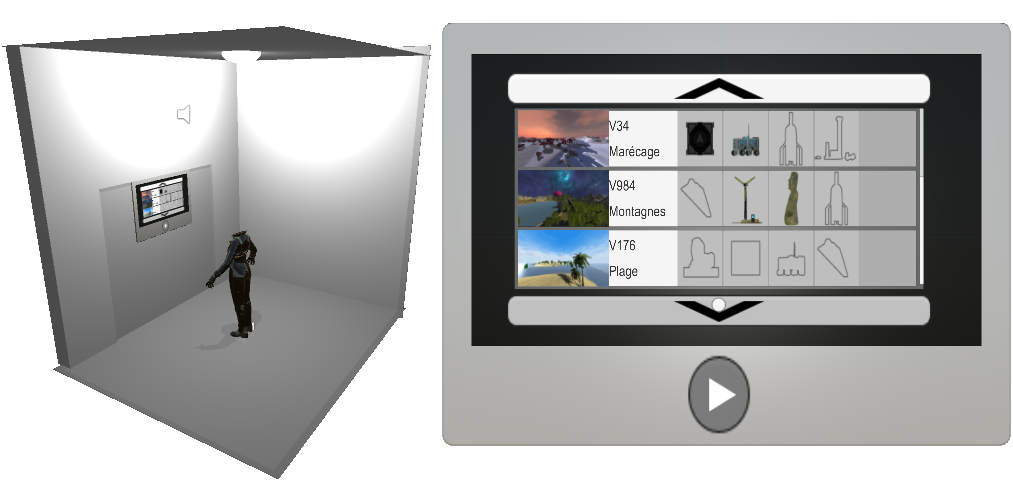
\includegraphics[height=\imgHeightSmall{}]{img/Results_LevelSelection.png}}
			\captionof{figure}{Pièce de choix des niveaux. À gauche: pièce contenant la lampe, le joueur, l'écran et une porte. À droite: écran de choix des niveaux, avec le curseur sur le bouton de défilement de la liste.}
			\label{LevelSelection}
		\end{minipage}\medskip	
	
		Le joueur ne peut pas avancer et peut uniquement choisir son niveau à l'aide d'un curseur situé au milieu du regard. Une liste déroulante des différents niveaux est affichée à l'écran. Le joueur peut naviguer dans cette liste à l'aide des boutons se trouvant en dessus et en dessous. Aucun clic n'est nécessaire, les boutons sont activés après un certain temps de survol. Le HMD permet de déplacer le regard et le joueur peut voir une représentation de son corps dans une tenue d'astronaute. Le modèle du joueur ne contient ni de casque ni de tête, ceci ne peut cependant pas être perçu par ce dernier. Son ombre contient le casque, donnant ainsi l'impression que l'avatar en porte un sans obstruer le champ de vision. Une fois le niveau sélectionné, le bouton \textit{play} s'active. Lorsque ce dernier est activé, la transition s'effectue (figure \ref{SceneTransition}).
		\\
		
		Une fois la transition achevée, la porte s'ouvre et le joueur voit une deuxième pièce (figure \ref{RoomAndHUD}). Dans cette pièce sont placés les différents éléments familiers (un bureau avec un ordinateur, une armoire, une fausse plante, une cadre et une photo de famille). Cette pièce contient également un autre personnage: le guide. Ce dernier effectue tout le parcours devant nous. Dès cet instant, le HUD est chargé et le joueur peut effectuer les différentes interactions. Ce HUD est placé en tant qu'enfant de la caméra. Il est placé devant elle et est orienté vers son centre (figure \ref{RoomAndHUD}). Une déformation est alors visible à l'écran mais l'effet est plus naturel avec le HMD. Ce HUD contient une carte du niveau montrant le chemin, l'emplacement du vaisseau et du joueur, la direction de son regard ainsi que les zones des objectifs à obtenir ou des points marquant ceux déjà obtenus. Le HUD contient également, en bas à droite, une barre d'oxygène représentant le temps restant. Elle se vide en allant du vert au rouge. D'autre éléments apparaissent à certains moment sur le HUD comme le \textit{scan} en cours ou encore un aperçu de l'objet ayant subi un \textit{scan}.\medskip		
	
		\begin{minipage}{\linewidth}
			\makebox[\linewidth]{
				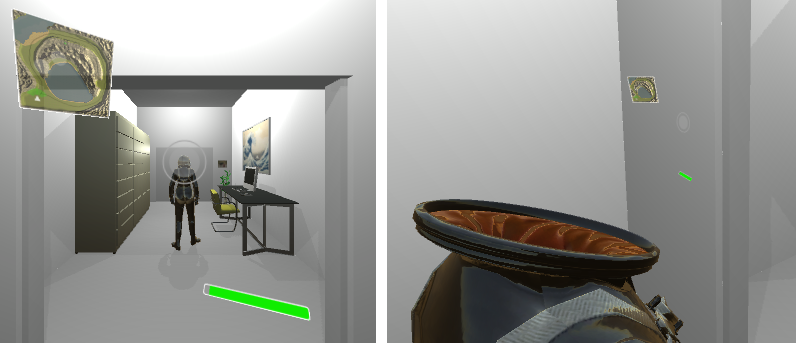
\includegraphics[height=\imgHeightSmall{}]{img/Results_Room.PNG}}
			\captionof{figure}{Deuxième pièce et HUD. À gauche: vision de la deuxième pièce depuis le point de départ avec le HUD affiché, un \textit{scan} du guide est en cours. À droite: vision de l'emplacement du HUD dans la scène.}
			\label{RoomAndHUD}
		\end{minipage}\medskip	
		
		Les différentes interactions sont les suivantes: le déplacement; le \textit{scan}; la pause. Le dernière étant possible uniquement en jouant sans LHS à l'aide de la touche "P". Pour le déplacement, il s'effectue avec le LHS ou au clavier s'il n'est pas disponible. La touche pour avancer est alors "W" ou "Flèche haut". La dernière interaction est le \textit{scan}. Il doit être effectué sur les objectifs et peut l'être sur le guide. Les différentes étapes du \textit{scan} sont détaillées dans la figure \ref{GuideScan}.
	
		Le joueur peut donc se déplacer pour traverser la pièce. L'avatar s'articule d'après les angles reçus du LHS ce qui induit le mouvement. Un simulateur contenant une animation de marche est utilisé pour ressortir ces angles quand le SG est joué au clavier. Le guide possède une animation de marche qui se lance quand le joueur s'approche. Il s'arrête et passe en animation d'attente qand le joueur est trop loin. La porte menant à la dernière pièce s'ouvre alors. Cette pièce est plus petite et fait office de sas. Elle ne contient qu'une lampe et une porte s'ouvrant différemment des autres (figure \ref{Spaceship}) et donnant sur l'extérieur. Ce n'est pas un sas au sens strict puisqu'il est possible qu'il ait ses deux portes ouvertes. Il sert cependant de passerelle entre l'environnement familier et la planète possédant un environnement étranger. C'est seulement une fois cette porte ouverte que l'on aperçoit le monde extérieur correspondant au niveau choisi. Une fois dehors, en se retournant, on peut visualiser le vaisseau dans lequel nous étions.
		\\
	
		Le joueur doit alors effectuer tout le parcours. La direction est automatique, il n'a qu'à avancer et essayer d'effectuer des \textit{scans} sur tous les objets lui semblant digne d'intérêt. Le but étant de trouver tous les objectifs. Ces derniers peuvent être répartit à gauche ou à droite du chemin d'après un paramètre donné par le thérapeute qui doit être récupéré de l'IHM. Des zones contenant les objectifs sont disponibles sur la carte du HUD. Les objectifs émettent également un scintillement sonore et un effet visuel de particules. La présence des zones, leur taille ainsi que l'activation du scintillement peut être choisit dans l'inspecteur du script "HelpModel" avant le lancement d'une partie. Dans le SG actuel, ces paramètres ne sont jamais modifiés.
		Une fois que le joueur a effectué tout le chemin, il rentre à nouveau dans le vaisseau. Il doit continuer d'avancer jusqu'à atteindre son point de départ. Un écran présente alors au joueur le score obtenu.
		\\
		
		Si le temps est écoulé ou que l'exercice est interrompu, une téléportation est effectuée pour placer le joueur devant cet écran. Cette téléportation va faire effectuer tout le chemin restant au joueur en trois secondes avec un effet de flou.
		
	\subsection*{Description des mondes}	
		Dans cette sous-section est décrit les cinq niveaux créés, leur environnement, leurs particularités ainsi que les \textit{landscape elements} qu'ils utilisent. Chaque niveau possède actuellement quatre objectifs dont un n'affichant des indications uniquement après qu'un certain nombre d'objectifs du niveau soient obtenus. Le temps à disposition pour chaque niveau est de 10 minutes.
		\\
		
		Le SG propose cinq niveaux différents. Les fonctionnalités du SG ont été créées à l'aide du premier monde. La tâche de création d'autres mondes a alors été attribuée à Monsieur K. Laipe. Il a alors créé quatre mondes (les mondes deux à cinq) avec, pour consignes, les contraintes de ces mondes et la volonté de créer des mondes plus vivants que le premier. Les terrains, leurs valeurs d'appauvrissement et le chemin de chacun de ces quatre mondes ont été créés par Monsieur K. Laipe. Il a trouvé les modèles des objectifs et \textit{landscape elements} utilisés. Il a également réalisé le placement et la paramétrage des objectif d'après les scripts existants. La génération des différentes géométries des \textit{landscape elements} a été réalisée par Monsieur K. Laipe. Il a également implémenté les animations, gérées par script, des vagues et des poissons (utilisés en décorations dans les mondes quatre et cinq).
		
		\begin{itemize}
			\item \textbf{Monde 1 --} C'est le premier monde qui a été créé, le temps minimum est de 6 minutes et 48 secondes. Il représente un canyon asséché (figure \ref{World1}). Sa \textit{skybox} montre une planète en fusion et des astéroïdes sur un fond noir avec des étoiles. Ses couleurs tendent vers le rouge et il est relativement sombre. Il ne possède aucun élément de décors ni sons d'ambiance. Il utilise quatre \textit{landscape elements}: le grand cristal; le petit cristal; la colonne de roche; le petit caillou. Les deux premiers sont rouges et de la même famille d'éléments. Les objectifs de ce niveau sont des outils ou parties de mécanismes. Dans l'ordre du parcours: une pioche; un rouage; un marteau; une hélice. Ce monde a servi de base pour l'implémentation des fonctionnalités et des premières démonstrations pour le mandant. La principale remarque était de créer, par la suite, des mondes plus riches en couleurs, plus lumineux et plus vivants. Remarque transmise à Monsieur K. Laipe pour la création des autres mondes. Ce monde a la particularité de contenir une petite pente car il a été développé avant que les pentes ne soient définies comme hors des objectifs de ce travail de Master;\medskip		
			
			\begin{minipage}{\linewidth}
				\makebox[\linewidth]{
					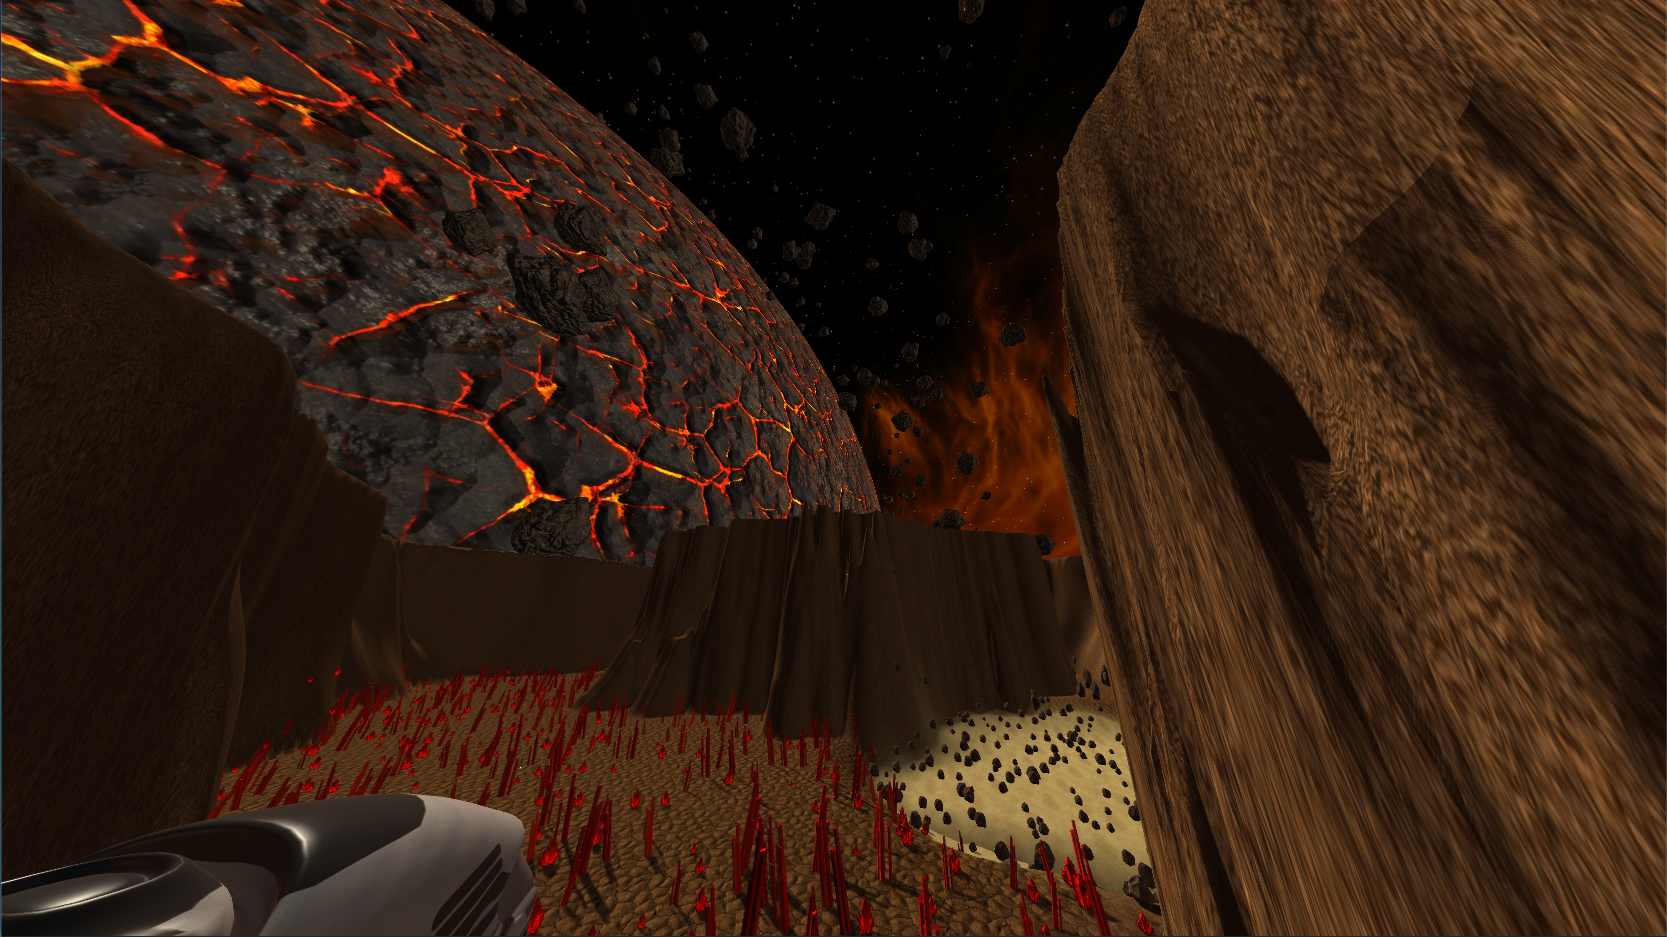
\includegraphics[width=\textwidth]{img/world1.PNG}}
				\captionof{figure}{Aperçu du monde 1.}
				\label{World1}
			\end{minipage}\medskip	%TODO: Refaire sans l'effet étrange et sombre
			
			\item \textbf{Monde 2 --} Il représente une rivière dans un paysage montagneux (figure \ref{World2}). Il dure au minimum 8 minutes et 29 secondes. Sa \textit{skybox} montre un ciel bleu nuageux avec de nombreuses étoiles visibles. Pour renforcer le sentiment de planète inconnue, deux planètes sont placées dans la scène. Leur couleur est atténuée et elles possèdent le script "ConstantDistanceController". Ce script permet, une fois le jeu dans l'état "PLAY" de garder une distance constante à la caméra, évitant ainsi que le joueur puisse remarquer qu'elles ne sont pas autant distantes qu'elles en ont l'air. Des plans d'eau ainsi qu'une cascade sont présents en tant que décors. La cascade émet un bruit d'ambiance. Trois \textit{landscape elements} sont utilisés: un arbre (sycomore); un buisson (Bush1); un caillou (Rock Planet2); Les objectifs sont les suivants: une éolienne (possédant une animation de rotation); un pont; une idole (ressemblant à un Moaï, les statues de l'île de Pâques); une statue de lion. Ce monde a la particularité de posséder un "PathModifier" permettant de modifier les bruit de pas et la hauteur d'un morceau de chemin (et de ne pas prendre ceux du terrain). Ce "PathModifier" est le pont, qui a la particularité d'être également un objectif. C'est le seul objectif qui possède la même position et orientation gauche et droite. Une autre particularité de ce monde est qu'il est le seul à avoir un parcours qui tourne majoritairement à gauche;\medskip		
			
			\begin{minipage}{\linewidth}
				\makebox[\linewidth]{
					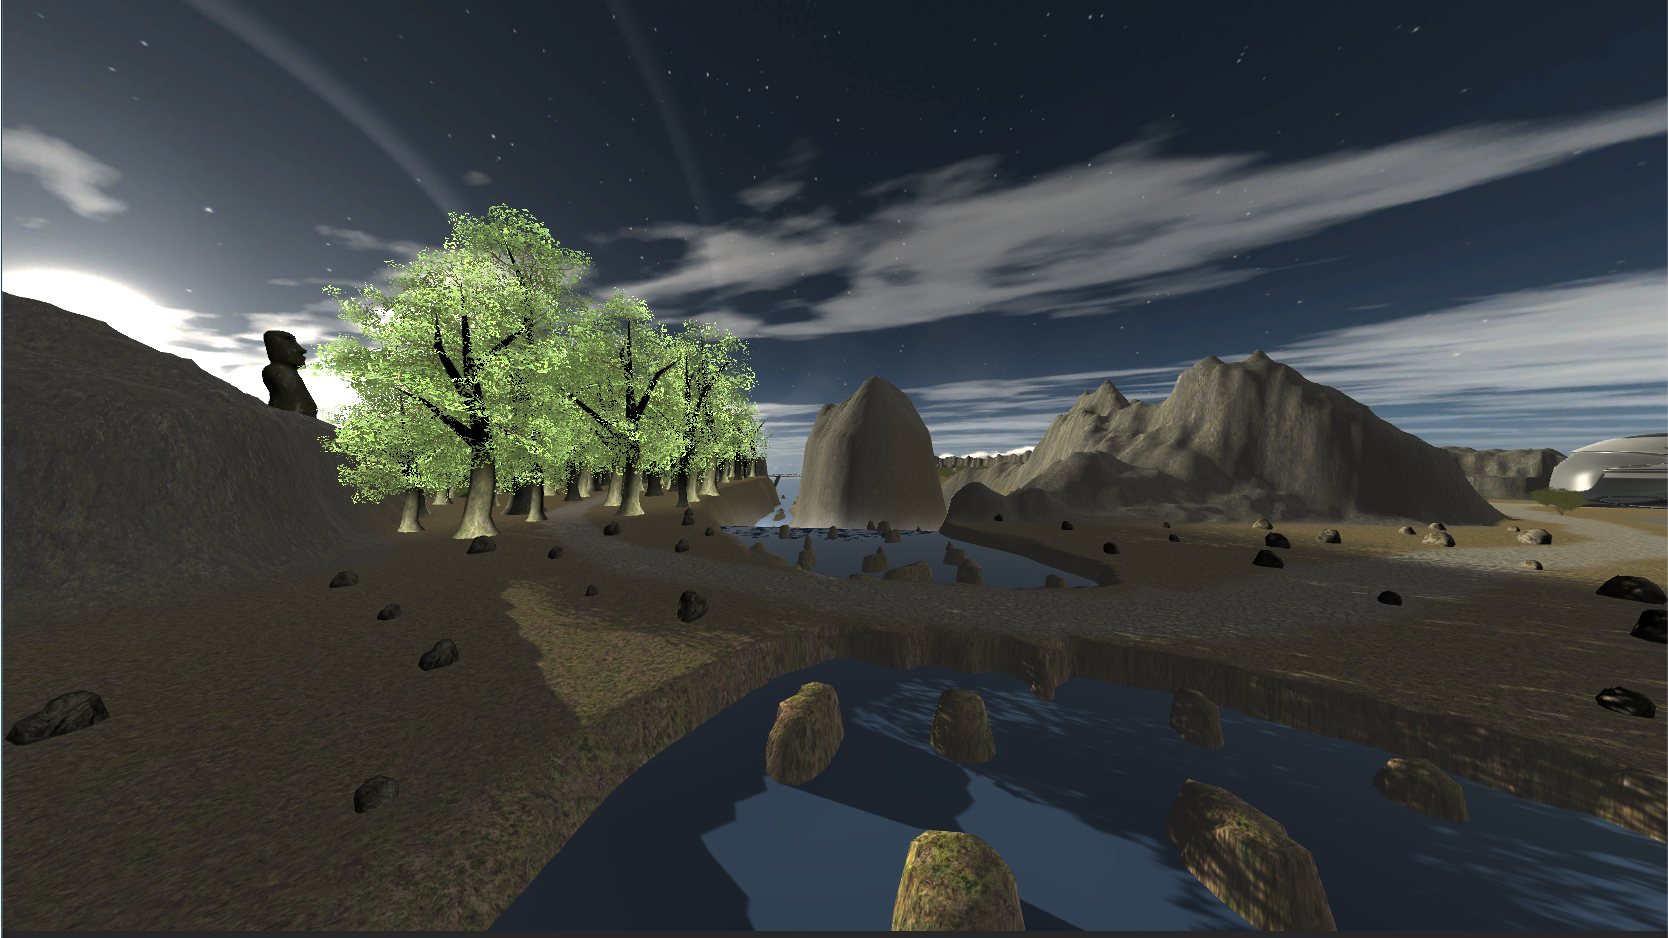
\includegraphics[width=\textwidth]{img/world2.PNG}}
				\captionof{figure}{Aperçu du monde 2.}
				\label{World2}
			\end{minipage}\medskip
			
			\item \textbf{Monde 3 --} Il représente des marécages enneigés (figure \ref{World3}). Il dure au minimum 8 minutes et 14 secondes. Sa \textit{skybox} représente un coucher de soleil sur une mer s'étendant jusqu'à l'horizon dans toutes les directions. Il possède un plan d'eau comme objet de décors, émettant un bruit d'eau vers les segments proches du chemin. L'ambiance de planète inconnue vient de la sélection de \textit{landscape elements}. Les cinq premiers étant les champignons du répertoire "Mushrooms" ayant tous le même style graphique mais étant de taille et composition différente. Les deux suivants sont un grand et un petit cristal violet. Le dernier est un érable japonais. Les objectifs sont: une caisse métallique; un petit véhicule robotisé; une tour métallique; des ruines. Ce monde a la particularité d'avoir un effet de particule sur tout le terrain. Cet effet représente de la neige qui tombe;\medskip		
			
			\begin{minipage}{\linewidth}
				\makebox[\linewidth]{
					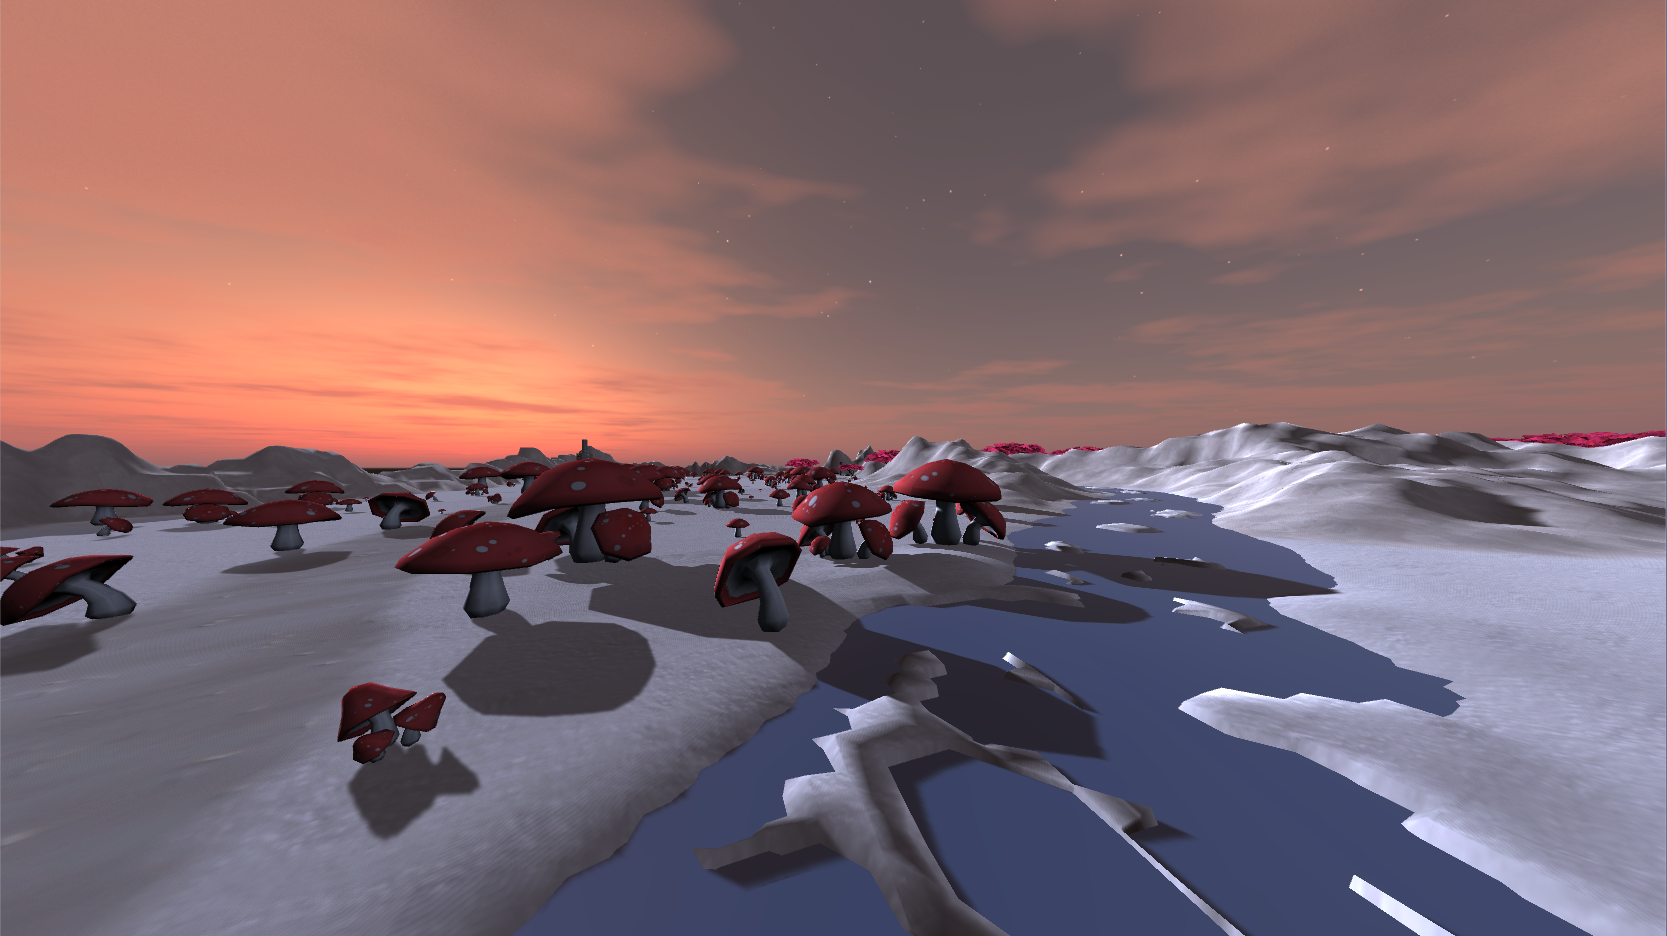
\includegraphics[width=\textwidth]{img/world3.PNG}}
				\captionof{figure}{Aperçu du monde 3.}
				\label{World3}
			\end{minipage}\medskip
			
			\item \textbf{Monde 4 --} Il représente un lac entouré de grandes collines (figure \ref{World4}). Il dure au minimum 8 minutes et 1 seconde. Sa \textit{skybox} montre une nébuleuse allant de bleu clair à violet. Il contient une planète rose et une étoile. La planète occupe une place importante dans le ciel alors que le soleil y est plus petit. Ils possèdent tous deux le script "ConstantDistanceController" (son rôle est expliqué dans la description du monde deux). Un plan d'eau est également présent avec un script l'animant verticalement pour donner un effet de vague. Dans le lac, quinze poissons sont présents. Ils possèdent une animation et un script contrôlant leurs déplacements. Ces \textit{landscape elements} sont: un saule pleureur; un petit bambou; un caillou (le même qu'au monde 2). Ses objectifs sont: un petit vaisseau spatial; une éolienne; une idole; une tour métallique. Ce monde ne possède pas d'autres particularités;\medskip		
			
			\begin{minipage}{\linewidth}
				\makebox[\linewidth]{
					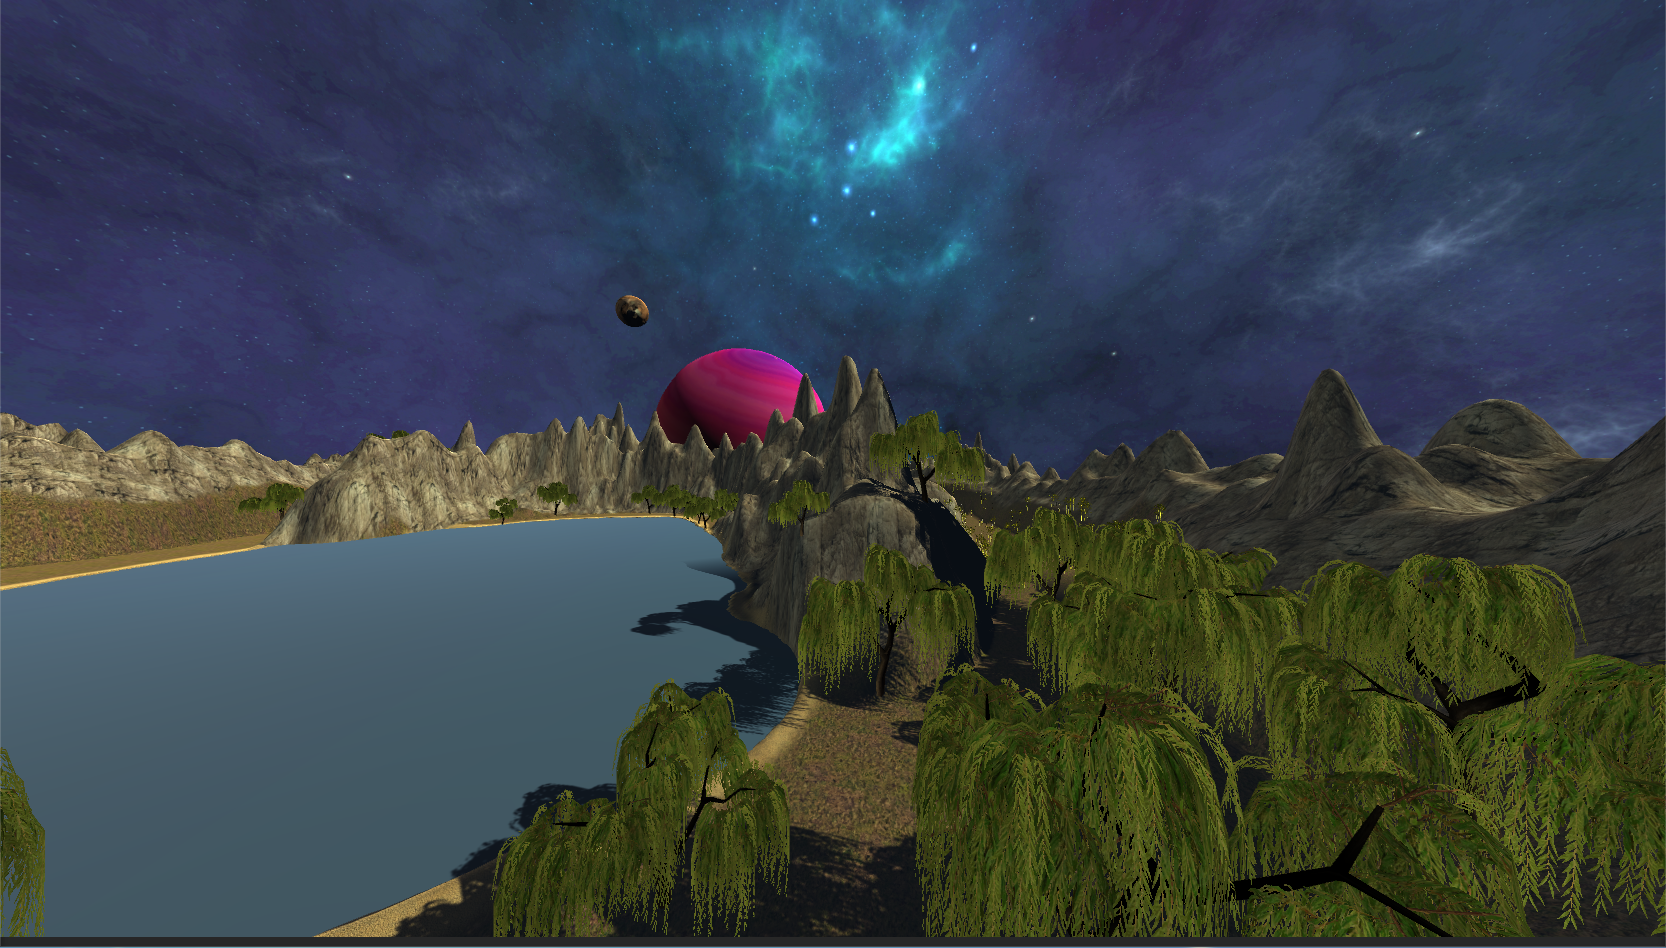
\includegraphics[width=\textwidth]{img/world4.PNG}}
				\captionof{figure}{Aperçu du monde 4.}
				\label{World4}
			\end{minipage}\medskip
			
			\item \textbf{Monde 5 --} Il représente une plage (figure \ref{World5}). Il dure au minimum 7 minutes et 48 secondes. Il possède une \textit{skybox} affichant un ciel bleu vif et des nuages blancs à l'horizon. Il possède, comme au monde 4, un plan d'eau et des poissons animés. Ces \textit{landscape elements} sont les suivants. Une famille de cinq palmiers possédant une animation pour leur feuillage. Une autre famille est également utilisées, elle est composée de cinq rochers verts pouvant représenter des structures de corail. Ces derniers ont un effet de surface réfléchissante. Les objectifs sont: une statue de lion; une boite métallisée; un petit véhicule robotisé; un petit vaisseau spatial. Ce niveau a pour particularité sont chemin qui effectue une forme de huit. C'est le niveau présentant le plus de courbes parmi tous ceux du SG.	\medskip		
			
			\begin{minipage}{\linewidth}
				\makebox[\linewidth]{
					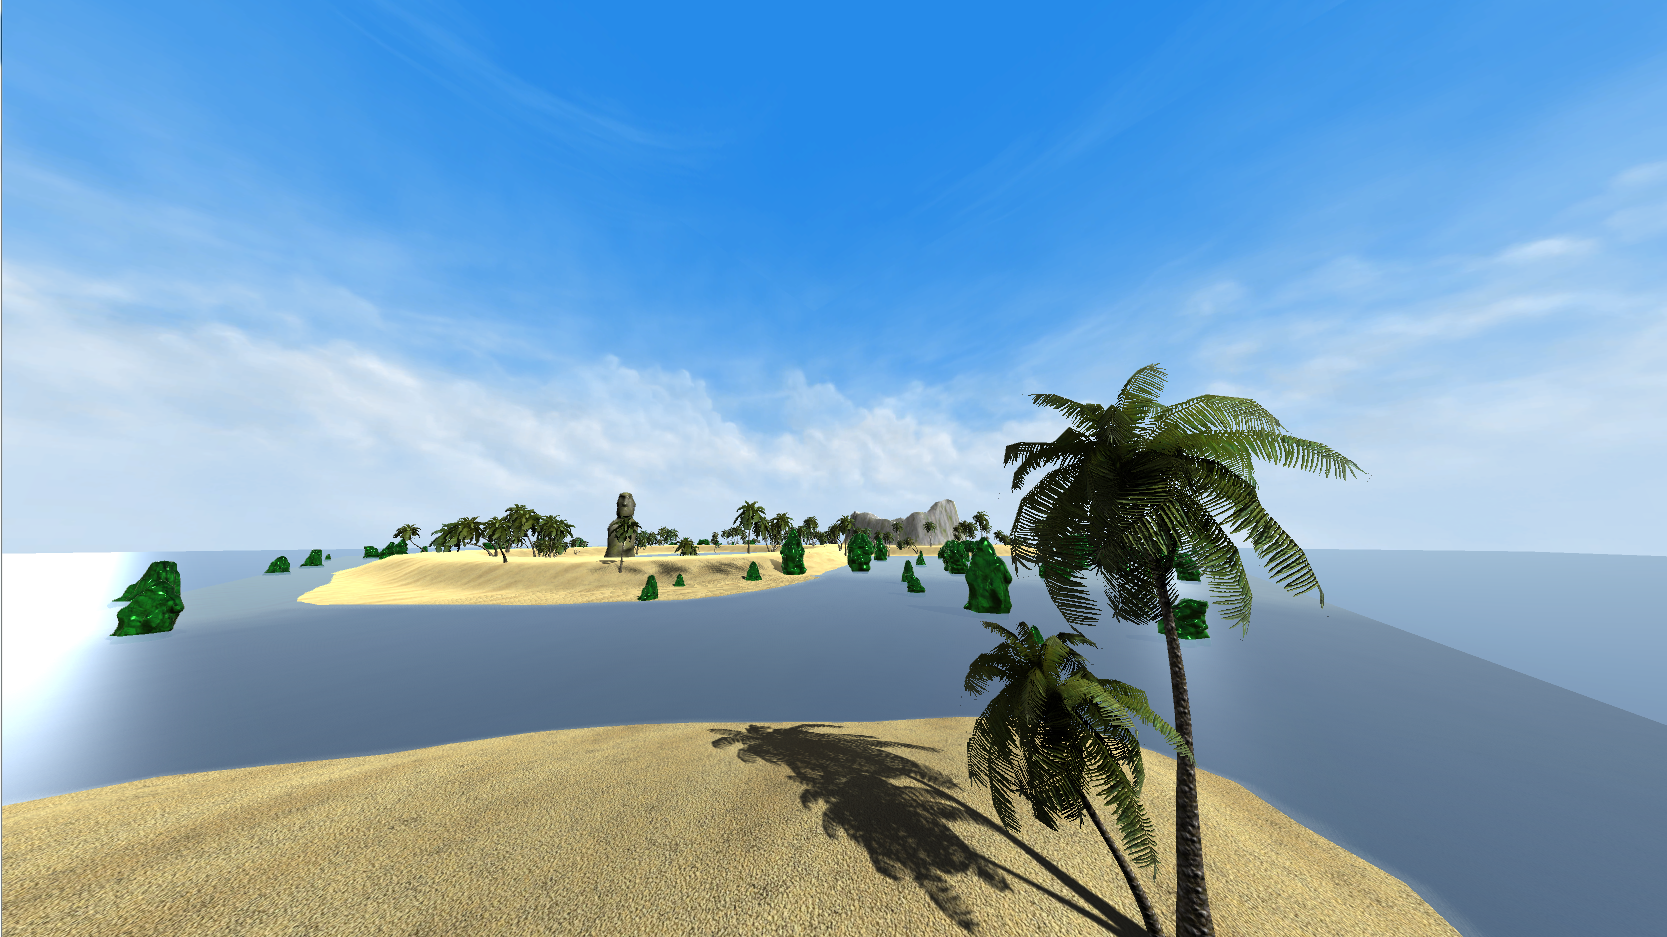
\includegraphics[width=\textwidth]{img/world5.PNG}}
				\captionof{figure}{Aperçu du monde 5.}
				\label{World5}
			\end{minipage}\medskip		
		\end{itemize}
		
		D'autres \textit{landscape elements} ont été créés (avec leurs différentes géométries) mais ne sont pas utilisés dans les niveaux. On peut en apercevoir, au parmi d'autres, dans la figure \ref{ObjectLibraryV2}.
		
	\subsection*{Appauvrissement}.
		Le SG propose neuf facteurs pour l'appauvrissement ainsi qu'un facteur général. Seul celui-ci doit être récupéré de l'IHM (en passant par l'application temps réel du LHS). Ce facteur assigne une valeur au neuf autres, comme il est possible de voir dans le tableau \ref{tableGeneralImpoverishment}. Ces neuf facteurs et leurs valeurs possibles sont résumés ci-dessous. Pour une description plus complète de leurs caractéristiques, de leur création et de leur implémentation, se référer à la section \ref{sDevAppauvrissement}.
		\begin{itemize}
			\item \textbf{Géométrie des \textit{landscape elements} --} Six valeurs possibles: géométrie totale; 2 \textit{billboards}; 2 \textit{billboards} avec normales; \textit{billboard}; \textit{billboard} avec normales; primitive 3D. Ces six valeurs sont visibles dans la figure \ref{DemoGeometryLandcapeElements};
			
			\item \textbf{Quantité des \textit{landscape elements} --} Correspond au paramètre "Quantity factor" dans l'inspecteur du script "ImpoverishmentModel". Est un nombre réel pouvant aller de 0 à 2. Le SG ne doit utiliser que les valeurs entre 0 et 1. Les valeurs supérieures étant prévues pour une surcharge d'objet. 0 correspond à aucun \textit{landscape element} et 1 à la quantité normale du niveau (pour un patient ne présentant pas de troubles cognitifs). L'évolution de la quantité est linéaire;
			
			\item \textbf{Géométrie du terrain --} Correspond au paramètre "Terrain details lvl" dans l'inspecteur du script "ImpoverishmentModel". Possède trois valeurs possibles: 1; 2; 3. La valeur 3 correspond au terrain tel qu'il est créé à la base. Les valeurs 2 et 1 proposent des versions sans rugosités, aux formes plus plates et géométriques;
			
			\item \textbf{Herbe --} Deux valeurs possibles: activée ou désactivée. L'herbe n'est pas obligatoire et est présente uniquement dans les mondes 2 et 3;
			
			\item \textbf{Animations --} Deux valeurs possibles: activées ou désactivées. Ne concerne pas les animations des portes, du guide et du joueur. Cet appauvrissement a été réalisé par M. Laipe avec, pour base, l'appauvrissement audio;
			
			\item \textbf{Particules --} Deux valeurs possibles: activées ou désactivées. Concerne tous les effets de particules, même ceux des objectifs (figure \ref{ParticlesImpoverishment}). Cet appauvrissement a été réalisé en parallèle de celui des animations par M. Laipe;
			
			\item \textbf{Effet de lumière --} Trois valeurs possibles: 0; 1; 2. Elles correspondent respectivement à une lumière unie; une lumière diffuse; une lumière diffuse avec des effets spéculaires (reflets). Tous les objets de la scène, sauf le terrain, sont modifiés pour posséder uniquement les effets de lumière choisis. L'effet uni éclaire les objets indépendamment des sources de lumière, il n'y a donc aucune ombre et les reliefs sont impossibles à percevoir. L'effet diffus supprime simplement tous les reflets. Le dernier effet correspond aux effets de lumière complets du SG;
			
			\item \textbf{Nombre de couleurs --} Ce paramètre indique le nombre de valeur que peut prendre chaque composante rouge, vert, bleu de chaque pixel à l'écran. Il va de 2 à 256. Son influence est difficilement perceptible, à moins de tomber dans de basses valeurs. Une fois perçue, on voit des zones de couleurs se créer à l'écran, notamment pour les ombres. Ces zones peuvent être interprétées comme de nouvelles géométries dans la scène qui devient alors difficilement interprétable. Pour cette raison, le résultat de cet appauvrissement n'est pas été jugé pertinent.
			
			\item \textbf{Audio --} Pour l'appauvrissement audio, les sons sont organisés en quatre familles: bruits de pas; sons d'interface; bruits d'ambiance; musique. La famille "sons d'interface" contient un son de succès lancé après le \textit{scan} d'un objectif ainsi que leur scintillement. Les sons d'ambiances sont tous des sons allant avec le décors ou le terrain (\textit{e.g.}, bourdonnement dans le vaisseau, bruit de cascade, etc.). L'appauvrissement est alors réalisé par la sélection des différentes familles. Un aperçu des différents sons par famille et de leurs emplacements est visible dans la figure \ref{AudioImpoverishment}.
		\end{itemize}
	
\section{Utilitaires développés}
	\label{sResUtilitaires}
	Pour la réalisation du SG actuel, de nombreux utilitaires ont été réalisés. Certains ont déjà été décrits avec le détail de leur utilisation tout au long du chapitre développement. Cette section regroupe la liste de ces utilitaires ainsi qu'un résumé de leurs fonctions.
	
	\subsection*{Actions supplémentaires}
		Le menu d'action de la fenêtre \textit{Unity} est enrichi pas des actions implémentées durant ce travail. Celles-ci se trouvent dans le menu d'actions "NWTools". Ces actions sont les suivantes:
		\begin{itemize}
			\item \textbf{InvertNormals --} Cette action permet d'effectuer une copie du \textit{mesh} sélectionné en lui inversant ses normales. Elle a été implémentée et utilisée pour l'importation de certains éléments qui possédaient des normales inversées (ce qui avait pour conséquence la vision de l'intérieur de l'objet plutôt que sa surface extérieure). Ce fut notamment le cas de certains objets de décors de l'environnement familier. La copie ainsi créée est sauvée dans "Assets/Meshes/Inverted/";
			
			\item \textbf{MergeMeshes --} Cette action permet de fusionner tous les \textit{meshes} d'un \textit{GameObject}. Elle fut utile pour la première version de placement des \textit{landscape elements}. Celle-ci les considérait comme des arbres du terrain \textit{Unity}. C'est ce dernier qui obligeait qu'ils soient en un seul \textit{mesh}. L'objet est créé dans le dossier "Assets/Prefabs/Landscape elements/\textit{selected object name}\_merged/";
			
			\item \textbf{Generate SinglePointBillboard --} Cette action est utilisée pour créer un \textit{billboard} à partir d'un \textit{billboard cloud} à une face. L'avantage principal du \textit{billboard} est qu'il s'oriente d'après la caméra. La création du \textit{billboard cloud} est expliquée plus loin dans cette section. Cette action est effectuée pour chaque la version "\textit{billboard}" et "\textit{billboard} avec normales" de chaque \textit{landscape element}. Pour créer l'objet voulu, il faut sélectionner l'objet préfabriqué du \textit{billboard cloud} modèle et lancer l'action. Le \textit{billboard} est alors créé dans le même dossier au nom de "BillboardSinglePoint" ou "BillboardSinglePoint\_n" si le modèle utilisé contenait des normales;
			
			\item \textbf{Terrain/Replace Splatmap --} Permet de remplacer la \textit{splatmap} d'un terrain par une texture donnée. La \textit{splatmap} est la texture décrivant l'utilisation des différentes textures du terrain. Cette action a été utilisée durant les tests de génération d'un terrain à partir d'un script Python \cite{python_website} en annexe. Ce script générait une \textit{heightmap} dans un fichier ".raw" ainsi que la \textit{splatmap} allant avec. L'action lance une boite de dialogue. Le champ "SplatMap" correspond à la texture étant à l'intérieur du terrain \textit{Unity} ciblé.
			Ce script a été trouvé sur le site d'un programme tiers permettant la création de terrain \cite{ReplaceSplatmap_sourceWebsite};
			
			\item \textbf{Terrain/Apply GameObjectMap --} Cette action permet la génération des \textit{landscape element} sur le terrain de la scène ouverte. Il faut sélectionner la texture "LandscapeElementsMap" du monde choisit avant de la lancer. Les éléments créés sont instanciés dans "World/Terrain/Landscape elements/";
			
			\item \textbf{Terrain/Export Splatmap --} Cette action permet d'exporter la \textit{splatmap} du terrain de la scène actuel (doit être sélectionné) en un fichier image. Celui-ci est créé dans le dossier "Assets" avec le nom "splatmap.png". L'exportation de cette image peut permettre de dessiner le parcours s'il suit une texture précise.
		\end{itemize}
		
	\subsection*{Autres utilitaires}
		Premièrement, les scènes "BillboardGenerator" et "ObjectiveViewGenerator", se trouvant dans le répertoire "Assets/Scenes/Tools", permettent la génération d'objets préfabriqués utiles au SG. Ceci grâce aux scripts du même nom que la scène concernée. Ces scripts utilisent des fonctionnalités de l'éditeur et ne peuvent être intégrés dans un \textit{build}. C'est pourquoi ils sont stockés dans le répertoire "Assets/Script/Editor". Cependant, pour s'en servir dans les scènes, ils doivent être temporairement sortit de ce répertoire. Ceci est dut au fait qu'ils n'agissent pas comme des actions présentes dans le menu d'actions mais doivent être attachés à un \textit{GameObject}. La première de ces scènes permet de générer les \textit{billboards cloud} à une ou deux faces, avec ou sans normales. Son fonctionnement est expliqué dans une sous-section de la section \ref{sDevAppauvrissement} du chapitre Développement. Les objets préfabriqués créés sont générés dans le répertoire "Assets/Prefabs/Landscape elements/Gen". La deuxième scène génère les images utilisées dans la sélection des niveaux comme aperçu des objectifs déjà obtenus. Son fonctionnement est similaire et l'image est générée dans le répertoire "Assets/Textures/UI/Objectives/Gen". À noter que la scène "ObjectiveViewGenerator" a été réalisée par Monsieur K. Laipe en s'inspirant de "BillboardGenerator". Il qui s'en est par servi par la suite pour créer les images des objectifs.
		\\
		
		Un script Python \cite{python_website} a également été créé durant la phase de tests de génération d'un terrain. Il a été décidé, suite à ces tests, que les terrains n'avaient pas à être générés pour ce travail. Ils peuvent donc être créés depuis l'éditeur de terrain \textit{Unity}. La génération de terrain étant tout de même un des aspects probables du projet R\&D englobant, ce script est conservé.

\section{Tests de performances}
	\label{sResTests}
	Sur la fin du travail, des tests de performances ont été réalisés sur le SG utilisé au clavier (l'intégration avec le LHS n'ayant pas pu être réalisée). Ces tests ont pour but l'identification de différents éléments nécessitant une optimisation pour la suite du projet.
	 
	Pour ces tests, un compteur d'images par secondes (\textit{fps}, de l'anglais \textit{frame per second}) est implémenté. Ce dernier est la classe "PerformanceModel" se trouvant dans l'objet préfabriqué "Models". Il permet de sauvegarder des métriques pour différents segments du déroulement d'une partie. Il enregistre ces métriques dans un fichier texte, à côté du fichier de persistance de progression du SG ("\%AppData\%/LocalLow/HEArc/SGTM/performances.txt"). Son avantage, comparé aux utilitairse \textit{Unity}, est qu'il compte réellement le nombre d'appels de la fonction "Update", appelée à chaque image \cite{Unity50Tips} et que ces métriques peuvent être réalisées depuis l'exécutable du SG. Ce dernier point permet de mesurer les performances effectives du SG sans la surcharge apportée par l'environnement \textit{Unity}.
	\\
	
	Les différentes métriques mesurées sont les suivantes: le nombre moyen d'images par seconde (\textit{fps}); le nombre d'images ayant nécessité plus de 50 ms de calcul; le nombre d'images hors du temps moyen nécessaire pour obtenir 30 \textit{fps}; le nombre d'images hors du temps moyen nécessaire pour obtenir 60 \textit{fps}; le temps maximum prit pour le calcul d'une image. Ces métriques sont sauvées pour: la scène de sélection des niveaux; la transition entre les scènes; la traversée de la pièce intérieure (jusqu'à ce que la porte du vaisseau d'ouvre); le parcours total du chemin. De façon générale, pour chaque étape, des balayages horizontaux et verticaux ont été réalisés pour simuler un regard explorant l'environnement. Pour le parcours total du terrain, des \textit{scans} des objectifs et du guide ont été réalisés. Ces mesures sont effectuées pour chaque niveau, avec le niveau d'appauvrissement général minimum (table \ref{tableGeneralImpoverishment}). Ce niveau d'appauvrissement est choisi car il possède le plus d'éléments avec la géométrie la plus riche. C'est donc l'appauvrissement nécessitant le plus de ressources. Ses métriques représentent donc le SG dans le cas d'utilisation le plus gourmand en ressources. La table \ref{tablePerformacnes} montre ces métriques. La limite des 50 ms correspond à la limite de la latence visuelle pour éviter de casser le sentiment de présence (chapitre "Analyse", section \ref{sAnaGameConceptPointsImportant}) \cite{Jay_RT_ModelingEffectsDelayedHaptic}. Les limites de 30 et 60 \textit{fps} sont choisies car elles sont les standards actuels pour les jeux PC \cite{PoweringTheRift}. Pour proposer une expérience optimale, il est souhaitable d'être au dessus de cette limite.\medskip
	
	\begin{minipage}{\linewidth}
		\begin{tabular}{|l|c|c|c|c|c|}
			\hline
			Métriques&	\textit{fps}& hors limite& hors limite& hors limite& temps\\
			& moyen& 60 \textit{fps}& 30 \textit{fps}& 50 ms& maximum [ms]\\
			\hline
			Sélection du niveau& 75& 0,8561\%& 0,0535\%& 0\%& 31,0\\
			\hline			
			Transition des scènes& 65& 3,5340\%& 1,5707\%& 1,1780\%& 312,0\\
			\hline
			Pièce intérieure& 58& 32,5243\%& 0,1477\%& 0,1055\%& 333,3\\
			\hline
			Terrain, monde 1& 68& 9,7335\%& 0,0152\%& 0,0076\%& 93,4\\
			\hline
			Terrain, monde 2& 64& 17,8751\%& 0\%& 0\%& 26,8\\
			\hline
			Terrain, monde 3& 37& 100\%& 0,0113\%& 0,0113\%& 80,0\\
			\hline
			Terrain, monde 4& 75& 0,0087\%& 0,0029\%& 0,0029\%& 53,4\\
			\hline
			Terrain, monde 5& 75& 0,003\%& 0,003\%& 0,003\%& 53,4	\\	
			\hline
		\end{tabular}
		\captionof{table}{Métriques mesurées sur les différentes étapes du SG et les différents niveaux.}
		\label{tablePerformacnes}
	\end{minipage}\medskip
	
	L'ordinateur utilisé pour la réalisation de ces tests possède les caractéristiques suivantes:
	\begin{itemize}
		\item \textbf{Processeur --} Intel Core I7-3930K, 6 cœurs, 3.20GHz;
		\item \textbf{RAM --} 16 Go;
		\item \textbf{Carte graphique --} NVIDIA GeForce GTX 680, taille mémoire 2Go;
		\item \textbf{Système d'exploitation --} Windows 7, 64 bits.
	\end{itemize}
	
	Les mesures pour les trois premières étapes on put être effectuées sur chaque niveau. Elles sont donc présentées  en moyenne dans le tableau \ref{tablePerformacnes}.
	
	On remarque qu'aucunes des étapes n'arrive à respecter constamment la contrainte minimale de 60 \textit{fps}. La traversée de la pièce intérieure possède presque un tiers de ces images ne respectant pas la contrainte des 60 \textit{fps}. Ceci est très probablement dû aux objets qui y sont présents. Ils ont été trouvés sur internet, libres de droit, mais possèdent par contre un nombre de sommets bien trop important pour leur utilisation dans ce SG (\textit{e.g.}, fausse plante > 100'000; armoire 2'210; ordinateur ~20'000; chaise > 5'000). Ces objets sont présents à titre de démonstration d'une pièce intérieure. Ces tests révèlent qu'une recherche plus approfondie de modèles plus légers, ou la modélisation de nouveaux objets devra être effectuée dans le projet R\&D englobant.
	\\
	
	On remarque aussi que la plupart des étapes mesurées ont eu une faible quantité d'images nécessitant plus de 50 ms de calcul. Ce point est problématique car cette valeur correspond à la limite avant de casser le sentiment de présence. Un travail général d'optimisation ou d'amélioration de la stabilité du SG est à effectuer pour réduire ce pourcentage à zéro. Cette tâche est d'autant plus grande que les valeurs mesurées ne prennent en compte que le calcul d'une image. Dans le SG final, ce temps ne sera pas entre l'intervalle de deux images, mais le temps entre l'interaction du patient et sa réponse à l'écran. Cela induit le temps nécessaire au LHS pour mettre à disposition cette variable ainsi que celui nécessaire à la récupération de cette variable par le SG.
	\\
	
	Si l'on regarde les différents niveaux, on note que le monde trois est le monde possédant les mesures les plus basses, avec aucune image calculée en dessous de la limite de 60 \textit{fps}. 
	Le nombre de sommets des objets utilisés peut également être mis en question: les champignons en ont de 154 à 616; l'érable en a 1'624; les cristaux en ont de 199 à 1'044. Une autre hypothèse est l'utilisation de l'herbe. Seule ce monde et le monde deux en utilisent. Le monde deux arrivant juste devant le monde trois avec une image sur six hors contraintes, cette hypothèse est probable. Ce monde est également le seul à posséder un effet de particules sur tout le terrain (neige). C'est donc également une cause probable.%TODO Comparer 1x sans landscape element, 1x sans particule et 1x sans herbe
	La dernière hypothèse vient de la comparaison avec le monde ayant les meilleures mesures: le monde quatre. Il a moins d'une image pour dix mille en dessous de ce seuil. Le monde quatre possède d'importants reliefs et il est difficile de pouvoir percevoir tout le terrain et ces éléments d'un seul point. Le monde deux quant à lui est un des mondes les plus plats. On y a constamment une vue d'ensemble sur tout le terrain et une majorité des \textit{landscape element} des différentes familles. Cette charge quantitative est la dernière hypothèse proposée.
	\\
	
	On remarque également que, pour la transition entre les scènes et la pièce intérieure, le temps maximum pour calculer une image est très grand (correspond à un \textit{fps} de 3). C'est probablement dû au chargement de la scène et à l'instanciation de tous les \textit{landscape elements}. Une solution pour effectuer ce chargement de façon asynchrone est à étudier.
	%TODO: Peut être dire que Kevin a bien testé le tout 
	%TODO: Pouvant être tester
	%Lag visuel ?
	%Interraction adéquate ?
	%Déplacement (astuce pied au sol reculant) convaicant ?

\section{Retour du domaine médical}
	\label{sResRetourDomaineMedical}
	Le SG actuel a été montré à un médecin cadre du Centre Hospitalier Universitaire Vaudois (CHUV), le Dr. Rolf Frischknecht. Il fait partie l'équipe du LHS en tant que conseiller médical et est en charge des aspects cliniques du LHS.
	Une description du SG et de ses principales fonctionnalités lui a été faite. Il a ensuite put tester le déroulement de niveaux entiers du SG ainsi que l'impact de chaque facteur d'appauvrissement. Cette section présente les principales remarques et critiques reçues sur le SG en général, les niveaux d'appauvrissement ou toutes autres remarques pouvant être utiles à la suite du projet. Les conséquences perçue de ses remarques et critiques y sont développées en tant qu'interprétation et non en tant que citation du Dr. R. Frischknecht.	
	
	\subsection*{Appauvrissement}
		Dans cette sous-section est décrit les principales remarques ayant été faite par rapport à l'appauvrissement de la scène. L'intérêt de ces remarques est de savoir si l'appauvrissement tel qu'il est présenté permet une interprétation facilité de l'environnement et diminue la charge cognitive. Les remarques du Dr. R. Frischknecht sont basées sur des notions de fonctionnement neuropsychologique obtenus en dehors de l’application de SG ou VR. Pour les vérifier dans le cadre de SG, il faudrait effectuer des tests cliniques spécifiques. Cependant, ces remarques peuvent être vues comme des pistes pour l'amélioration de cet appauvrissement.
		\\
		
		Les remarques concernant l'appauvrissement géométrique des \textit{landscape elements} sont les suivantes. La modélisation à l'aide de primitives 3D semble être pertinente. La complexité visuelle de l'objet est nettement diminuée mais il est tout de même reconnaissable. La pertinence des \textit{billboards} ou \textit{billboards clouds} est moins certaine. Il est tout de même intéressant de conserver ces géométries tant que des tests plus poussés n'ont pas été effectués.
		\\
	
		Pour l'appauvrissement du nombre de couleurs, il a été confirmé qu'il n'est pas souhaitable tel qu'il est implémenté. La suppression des nuances de couleurs n'aide pas à diminuer l'effort d'interprétation. Au contraire, la création de zones de couleurs fusionnant les différentes ombres complique l'interprétation des géométries.
		\\
		
		Pour l'appauvrissement des effets de lumière, il a été remarqué que la valeur minimum "effet lumière unie", dans certaines situations, complique l'interprétation. C'est le cas lors de l'utilisation des primitives 3D qui n'utilisent pas de texture mais une couleur, ou encore de certains \textit{billboards} sans normales (notamment les cristaux). Quand ceux-ci se superposent à l'écran, il est alors difficile de comprendre leurs formes. Cette valeur d'appauvrissement est cependant à conserver et semble, en dehors de la situation donnée, demander moins de travail d'interprétation. L'ajout de contours sur les objets pourrait permettre de résoudre ce problème.
		\\
		
		Finalement, trois critères principaux pour l'appauvrissement sont ressortis: quantité; richesse; diversité. Il est suggéré de ne pas utiliser un seul paramètre d'appauvrissement pour l'IHM mais deux. L'un agissant sur la quantité et l'autre sur la complexité (richesse). Il peut être intéressant pour la suite du projet de considérer un appauvrissement de la diversité, le seul critère non traité actuellement.
		
		De façon générale, un modèle simplifié peut devenir trop abstrait et demander paradoxalement un effort supplémentaire pour son interprétation. La facilité d'interprétation peut être vue comme une fonction parabolique de la complexité. Le but est d'en trouver son point minimum.		
	
	\subsection*{Remarques pour l'héminégligence}
		Dans cette sous-section sont décrites les principales informations reçues concernant l'héminégligence et le potentiel du SG pour des patients souffrant de tel trouble cognitif.
		
		L'héminégligence concerne le plus souvent le côté gauche. Il est tout de même souhaitable que ce côté puisse être réglé dans le SG. Cependant, si des aspects doivent être définis de façon définitive d'un côté ou de l'autre, il faudra favoriser une réalisation pour l’héminégligence gauche pour concerner le plus de personnes.
		
		Un autre phénomène existe chez les patients souffrant d'héminégligence: l'hémiextinction. Ce terme désigne la non perception d'un stimulus du côté négligé quand un autre stimulus est présent du côté sain, alors qu'il serait perçu s'il était seul. Concernant le SG, il faut alors veiller que les objectifs placés du côté négligé le soient à un endroit où le côté sain est pauvre ou abondant en stimuli pour une difficulté respectivement faible ou grande.
		\\		
		
		Durant la démonstration, il a été dit que le SG pourrait trouver son utilité même sans le LHS. Dans son état actuel, il permet l'appauvrissement ou l'enrichissement d'une scène et propose un challenge, même si le déplacement est automatique ou induit par une touche du clavier. Il peut être envisagé de l'utiliser pour évaluer l'état cognitif de patients souffrant d'héminégligence ou pour réapprendre progressivement à considérer le côté négligé. La création de métriques liées aux mouvements effectués par la tête ou encore un score pour chaque côté (comme évoqué dans l'analyse) semble être potentiellement d'une grande valeur pour les thérapeutes.
		
		Pour pouvoir efficacement être utilisé dans ces conditions, une fonctionnalité supplémentaire a été évoquée. Celle-ci peut également apporter une valeur au SG utilisé avec le LHS. Elle concerne la visibilité des objectifs. Il serait souhaitable de pouvoir augmenter la taille ou la visibilité (intensité des couleurs) des objectifs du côté négligé. Cette augmentation doit être paramétrable. Un ratio entre taille ou visibilité des objectifs du côté négligé par rapport aux autres peut ainsi être créé. La valeur de ce ratio lorsque le patient arrive à identifier un objectif dans son côté négligé peut être une métrique utile aux thérapeutes. Cette augmentation pourrait aussi intervenir temporellement et s'effectuer progressivement lorsque l'objectif est à portée de vue. Le temps nécessaire à sa détection peut alors déterminer ce ratio. 
		
		Une autre fonctionnalité a été évoquée: guider le joueur vers l'objectif. Si celui-ci est du côté négligé, on pourrait guider le regard à l'aide d'un flux allant du côté sain au côté négligé. Le joueur n'aurait donc qu'à suivre ce flux pour arriver à l'objectif. La densité de ce flux doit être paramétrable et peut également évoluer dans le temps et donner une métrique supplémentaire. Ce flux pourrait être artificiel tel que des flèches placées sur le HUD du joueur. Ou alors être naturel comme un vol d'oiseaux, des poissons dans un cours d'eau ou des feuilles soufflées par le vent.
	
	\subsection*{Autres remarques}
		D'autres remarques ont été faites sur le SG actuel. Premièrement, il serait souhaitable de synchroniser les mouvements du guide avec ceux du joueur. Ceci afin de renforcer les chances de solliciter correctement les neurones miroirs et ainsi espérer améliorer la réhabilitation. Si les mouvements du joueur sont guidés ou corrigés par le LHS, le guide peut alors être articulé de la même façon que l'avatar. Il faut en conséquence revoir sa logique de déplacement pour plus qu'il ne s'arrête pas et que sa distance soit plus constante. Si les mouvements du joueur sont libres, il faut alors trouver le moyen d'en extraire un rythme et de synchroniser la marche du guide sur celui-ci.
		\\
		
		Finalement, des "clignotements" ou "frétillements" autours de certains \textit{landscape elements} tels que les arbres ou encore liés à la lumière ont été perçus. Ceux-ci peuvent être dû à la résolution du HMD, aux calculs d'éclairage ou seraient le résultat de tâches de la carte graphique entre les \textit{shader}, tel que le "\textit{clipping}" or la "rastérisation" \cite{Gobron_WebGL}. Ces tâches étant le tri et la sélection des pixels utilisés.
		Ces clignotements ont été identifiés comme surchargeant inutilement le cerveau. Il est souhaitable d'en trouver la raison exacte ainsi qu'un moyen de les supprimer.
		
		
	
	
	
	
	